\documentclass[aps,prl,reprint,groupedaddress]{revtex4-1}
\usepackage{graphicx}

\begin{document}

%Title of paper
\title{Molecular Dynamics under Lennard-Jones potential}


\author{Eduardo Pavinato Olimpio}
%\email[]{epolimpio@gmail.com}

\affiliation{ICCP - Delft University of Technology}

\date{\today}

\begin{abstract}
% insert abstract here
	In this report we outline the results obtained using a classical molecular dynamics model for atoms interacting under the Lennard-Jones potential. The simulations were run using values compatible to the dynamics of Argon atoms as done by \textit{Verlet} \cite{Verlet1967}. We use the simulation to calculate the pressure, the heat capacity and the correlation function of this system for different temperatures and volumes. Moreover, for the liquid phase, we reproduce the results of \textit{Alder \& Wainwright} \cite{Alder1970} which shows that the decay of the velocity autocorrelation goes as the power $-3/2$ with time.
\end{abstract}

\maketitle

% References should be done using the \cite, \ref, and \label commands
\section{Introduction}
% Put \label in argument of \section for cross-referencing
%\section{\label{}}
Molecular dynamics has been successfully used method for studying classical many-particles systems. It has been used for the study of systems in equilibrium and also for the understanding of the behavior out of equilibrium \cite{RapaportBook}. The methodology behind the simulation is simple and consists on integrating the classical equation of motion ($\vec{F} = m\vec{a}$) through time. However, there are some subtleties used for the computation of the problem which will be explained in the next section.

In the reported simulations, both the number of particles and the system volume are kept constant. And, as a result of the fact that the forces depend only on the relative positions of the particles, both the total momentum and energy of the systems are  constant, which implies that this is equivalent to a microcanonical ensemble.

The physical quantities of the system are obtained through the calculation of the ensemble averages. Therefore, we need to use a reasonable number of particles in the simulations. In our simulations we use 864 particles in line with the literature \cite{Verlet1967, Rahman1964}.

In the following sections we describe the methods employed in the simulation of the molecular dynamics under the Lennard-Jones potential. Subsequently, the thermodynamic quantities and the correlation functions are presented. Finally, we discuss about the decay of the velocity autocorrelation function.

\section{Simulation description \label{description}}

The simulation approach used follows closely the description of section 8.2-4 of the book of \textit{Thijssen} \cite{ICCPBook}. As mentioned before, we consider that the particles interact through the Lennard-Jones potential:

\begin{equation}
	V(r) = 4 \epsilon \left[\left(\frac{\sigma}{r} \right)^{12} - \left(\frac{\sigma}{r} \right)^{6} \right]
\end{equation}

In all the simulations we follow the approach of \textit{Verlet} \cite{Verlet1967} and use natural units, with $\epsilon = 1$, $\sigma = 1$, $m = 1$ and the Boltzmann constant $k_B = 1$. Hence, all lengths are given in units of $\sigma$, the energies are in units of $\epsilon$ and the temperature in units of $\epsilon/k_B$. For argon, $\sigma = 3.405 \textup{\AA}$, $\epsilon/k_B = 119.8 \textup{K}$ \cite{Argon} and $m = 39.948 \textup{u}$. Using natural units we can write the force between two particles as:

\begin{equation}\label{force}
	\vec{F_{ij}} = 24 \left( \vec{r_i} - \vec{r_j} \right) \left(2r_{ij}^{-14} - r_{ij}^{-8} \right)
\end{equation}
where $r_{ij} = |\vec{r_i} - \vec{r_j}|$. The force over each particle is calculated as the sum over all the pairs of the force acting over it. However, we apply a cutoff distance over which we consider that the force vanishes. This is reasonable looking at the form of the force, which decays as $r^{-8}$ for long distances. In accordance to the literature we choose the cutoff distance as $r_{c} = 3.3 \sigma$ \cite{Verlet1967, ICCPBook}, but we do not include in our simulation a neighbour list.

With the force, to calculate the motion of the particles we need an integration method for the second order equation we need to solve ($\vec{F} = m\ddot{\vec{r}}$). This is accomplished by the use of the \textit{Verlet Algorithm}. We outline below how the algorithm is implemented. For the details regarding the theory behind it, we recommend the reader to look at Sections 8.4 and A.7.1 of \textit{Thijssen} book \cite{ICCPBook}. Using a time step $h$, the update of positions and velocities are done by:

\begin{equation}
\begin{array}{l l}

\vec{v}(h/2) = \vec{v}(0) + \vec{a}(0)\frac{h}{2} \\
\vec{r}(h) = \vec{r}(0) + \vec{v}(h/2)h \\
\text{Calculate $\vec{a}(h)$ using $\vec{r}(h)$} \\
\vec{v}(h) = \vec{v}(h/2) + \vec{a}(h)\frac{h}{2}

\end{array}
\end{equation}

It is important to point out that the accumulated error in position after a large number of integration steps is $\mathcal{O}(h^2)$. The same holds true for the velocity. Although better precision algorithms could be implemented, the \textit{Verlet algorithm} has the advantage of being simple and stable. Most important, the algorithm is time reversible, which warranties that the integrator will not lead to energy drift (arithmetic errors can lead to drift for long times). This is a property of the more general concept of \textit{sympletic integrators}, which has the property of generating solutions with the same geometric properties in phase space as the continuum dynamical system. The \textit{Verlet algorithm} is the simplest implementation of this class of integrators. It can be seen from Table \ref{thermo_data} that the total energy per particle oscillates in the fifth digit, indicating the stability of the algorithm.

\subsection{Initial conditions}

In addition to the number of particles, we set the temperature ($T$) and the density ($\rho = N/V$) of the system in natural units. Given these conditions, the velocities are set in a Gaussian distribution (in each direction) with zero mean, such that the total momentum is zero. The standard deviation of the velocity distribution (in a defined direction, e.g., x) is given by the mean of the kinetic energy:

\begin{equation}
	\frac{1}{2}m \langle v_x^2 \rangle = \frac{1}{2}  k_B T 
\end{equation}

The initial positions are such as that the particles are located in the sites of a Bravais-FCC lattice, which is the ground state configuration of the noble gases such as Argon \cite{ICCPBook}. For each unit cell, we have 4 particles. Moreover, as we use a box of M cells per length, the number of particles is chosen such that the FCC configuration is completed, therefore $N = 4M^3$. For our simulation we use $M=6$ such that $N=864$.

As the simulation starts, however, the system relax towards equilibrium, which changes the total kinetic energy of the system, and consequently its temperature. As we want the temperature to be close to the temperature we set, for the initial time steps we renormalize the velocities of all the particles as:

\begin{equation}
	\vec{v_i}(t) \to \lambda \vec{v_i}(t) \quad \text{with} \quad \lambda = \sqrt{\frac{(N-1)3k_BT_{\text{set}}}{\sum_i mv_i^2}}
\end{equation}
where $T_{\text{set}}$ is the temperature we set. The system keeps drifting from the set temperature until it relax towards equilibrium and the renormalization process is kept during the initial part of the simulation (which is not used for the calculation of the physical quantities). In our case we apply the first renormalization after 300 time steps and, subsequently, we renormalize 30 times every 25 time steps. For the conditions in which we run our simulations, this is enough to let the system reach equilibrium in the set temperature. It is worth to note that, as the system is in a microcanonical ensemble, the temperature will oscillate around the the set value, and the mean is close, but not equal, to the set temperature, as shown in Table \ref{thermo_data}.

\subsection{Choice of the time step}

In natural units, the time is given in units of $\tau = \sqrt{m \sigma^2/\epsilon}$ which, for Argon atoms, is equal to $2.156 \textup{ps}$. Approximating the Lennard-Jones potential as an harmonic potential around the minimum, we can estimate the oscillation frequency. This is given by $\omega^2 = \frac{72 \epsilon}{m 2^{1/3} \sigma^2}$, which means that the period of oscillation is $T \approx 0.83 \tau$. Hence, we need to choose the time step to be a small fraction os this period. In our simulations we use $h = 0.004 \tau$, which is around $5 \%$ of the period and is around $10^{-14} \textup{s}$ for argon, in line with the literature \cite{Rahman1964}. After the temperature stabilization, we run the simulation for $10^4$ time steps, which means that it runs for $10^{-10} \textup{s}$

\subsection{Periodic boundary conditions}

We deal with the boundaries assuming periodic boundary conditions. This means that when a particle crosses the boundary of the system it comes in by the opposite side with the same velocity vector. It can be thought as if the system had copies of it around the box which means that we have to take the boundary into account in the calculation of the distances $r_{ij}$ in equation \ref{force}. We can notice that, being the box of size $L$, the maximum distance between the particles in one direction is $L/2$.

\section{Thermodynamic Quantities \label{thermo}}

\begingroup
\squeezetable
\begin{table}[ht]%[H] add [H] placement to break table across pages
\caption{Thermodynamic data extract from simulation\label{thermo_data}}
\begin{ruledtabular}
\begin{tabular}{ c  c  c  c  c  c }
$\rho$ & T (set) & T (real) & $U$ & $\beta P/\rho$ & $C_{\text{pot}}/N$ \\ \hline
0.3 & 1.5 & 1.48(2) & 0.14201(2) & 0.48(1) & 0.1991(7) \\ 
0.3 & 2.0 & 1.983(3) & 1.04749(2) & 0.8(1) & 0.1613(4) \\ 
0.3 & 3.0 & 2.984(4) & 2.72418(3) & 1.11(1) & 0.132(2) \\ 
0.45 & 1.0 & 1.066(2) & -1.76739(4) & -0.21(2) & 0.354(3) \\ 
0.45 & 1.25 & 1.267(2) & -1.22426(2) & 0.14(2) & 0.286(2) \\ 
0.45 & 1.5 & 1.503(3) & -0.73728(2) & 0.49(2) & 0.293(2) \\ 
0.45 & 2.0 & 2.004(3) & 0.17443(3) & 0.97(2) & 0.255(1) \\ 
0.45 & 3.0 & 2.98(5) & 1.87608(4) & 1.4(1) & 0.2162(9) \\ 
0.6 & 1.0 & 1.025(2) & -2.6561(2) & -0.35(2) & 0.511(9) \\ 
0.6 & 1.25 & 1.265(3) & -2.16172(2) & 0.38(2) & 0.493(8) \\ 
0.6 & 1.5 & 1.482(3) & -1.73153(2) & 0.82(2) & 0.415(5) \\ 
0.6 & 2.0 & 1.983(4) & -0.76583(3) & 1.45(2) & 0.351(3) \\ 
0.6 & 2.5 & 2.497(5) & 0.20524(4) & 1.79(2) & 0.339(3) \\ 
0.6 & 3.0 & 3.026(5) & 1.19484(5) & 2.01(2) & 0.314(2) \\ 
0.75 & 0.75 & 0.746(2) & -4.2838(1) & -1.2(3) & 0.73(2) \\ 
0.75 & 1.0 & 1.001(2) & -3.69718(1) & 0.52(2) & 0.67(2) \\ 
0.75 & 1.25 & 1.267(3) & -3.0989(2) & 1.51(2) & 0.67(2) \\ 
0.75 & 1.5 & 1.513(3) & -2.56276(2) & 2.05(2) & 0.58(1) \\ 
0.75 & 2.0 & 1.999(5) & -1.52344(3) & 2.67(2) & 0.55(1) \\ 
0.75 & 2.5 & 2.529(6) & -0.40984(5) & 2.99(2) & 0.56(1) \\ 
0.75 & 3.0 & 2.98(7) & 0.51513(6) & 3.14(2) & 0.54(1) \\ 
0.88 & 0.5 & 0.502(1) & -6.125036(6) & -6.27(3) & 1.07(6) \\ 
0.88 & 0.75 & 0.748(2) & -5.447434(8) & -1.38(3) & 1.16(8) \\ 
0.88 & 1.0 & 0.99(3) & -4.45755(1) & 3.01(3) & 1.07(7) \\ 
0.88 & 1.25 & 1.236(3) & -3.82496(2) & 3.79(2) & 0.88(4) \\ 
0.88 & 1.5 & 1.505(4) & -3.15495(2) & 4.24(2) & 0.81(3) \\ 
0.88 & 2.0 & 1.998(5) & -1.96305(4) & 4.64(2) & 0.73(2) \\ 
0.88 & 2.5 & 2.426(6) & -0.95865(5) & 4.78(2) & 0.73(3) \\ 
0.88 & 3.0 & 3.037(8) & 0.43967(8) & 4.83(2) & 0.74(3) \\ 
1.0 & 0.5 & 0.495(1) & -6.915778(4) & -0.65(3) & 1.4(1) \\ 
1.0 & 0.75 & 0.743(2) & -6.224198(8) & 2.22(3) & 1.12(7) \\ 
1.0 & 1.0 & 1.001(3) & -5.51146(1) & 3.65(3) & 1.3(1) \\ 
1.0 & 1.25 & 1.243(4) & -4.84508(2) & 4.43(3) & 1.3(1) \\ 
1.0 & 1.5 & 1.475(4) & -4.18722(2) & 4.98(3) & 1.3(1) \\ 
1.0 & 2.0 & 2.029(6) & -1.91352(5) & 7.6(3) & 1.04(6) \\ 
1.0 & 2.5 & 2.558(7) & -0.53304(7) & 7.39(3) & 0.92(5) \\ 
1.0 & 3.0 & 3.013(8) & 0.61486(9) & 7.18(3) & 0.88(4) \\ 
1.2 & 0.5 & 0.511(2) & -6.657415(9) & 25.1(8) & 1.4(1) \\ 
1.2 & 0.75 & 0.747(2) & -5.97515(1) & 19.64(6) & 1.3(1) \\ 
1.2 & 1.0 & 0.999(3) & -5.25261(2) & 16.62(5) & 1.3(1) \\ 
1.2 & 1.25 & 1.257(4) & -4.51718(3) & 14.75(5) & 1.2(9) \\ 
1.2 & 1.5 & 1.491(4) & -3.85472(4) & 13.6(5) & 1.3(1) \\ 
1.2 & 2.0 & 1.987(6) & -2.45871(6) & 12.03(4) & 1.19(9) \\ 
1.2 & 3.0 & 3.049(9) & 0.6032(1) & 10.48(4) & 1.4(1) 
\end{tabular}
\end{ruledtabular}
\end{table}
\endgroup

\subsection{Pressure}

The pressure is calculated through the virial expansion, with a correction for the fact that we have a cutoff distance ($r_c$) in the calculation of the force \cite{ICCPBook}:

\begin{equation}
\begin{array}{r r}
  \frac{PV}{N k_B T} = 1 - \frac{1}{3Nk_BT}\left\langle \sum_i \sum_{j>i} r_{ij} \frac{\partial U}{\partial r_{ij}} \right\rangle_{r_c} \\
   - \frac{2\pi N}{3k_BTV}\int_{r_c}^{\infty} r^3 \frac{\partial U}{\partial r} g(r) dr
\end{array}
\end{equation}
where the derivative of the potential is given by the force, $-F_{ij}$. Following the approach of \textit{Verlet} \cite{Verlet1967}, for the correction term we use $g(r) = 1$ above the cutoff, such that the correction will be given by:

\begin{equation}
  \int_{r_c}^{\infty} r^3 \left[ 24 \epsilon \left( -\frac{2 \sigma^{12}}{r^{13}} + \frac{\sigma^6}{r^7} \right) \right] = 8 \epsilon \left( -\frac{2 \sigma^{12}}{3r_c^{9}} + \frac{\sigma^6}{r_c^3} \right)
\end{equation}

The values obtained for several conditions are reported on Table \ref{thermo_data} and Figure \ref{press_graph}. For an ideal gas the \textit{compressibility factor} $\beta P/\rho$ is 1. Indeed, for low densities and high temperatures, the values obtained are close to 1. Another feature that is clear from the data is the following: if the particles has a mean distance that the dominant forces are attractive, the ratio is below 1 (possibly negative for high attraction); if the particles tend to stay closer to each other (high temperature and/or high density), then the compressibility factor is above 1.

\begin{figure}[ht]
	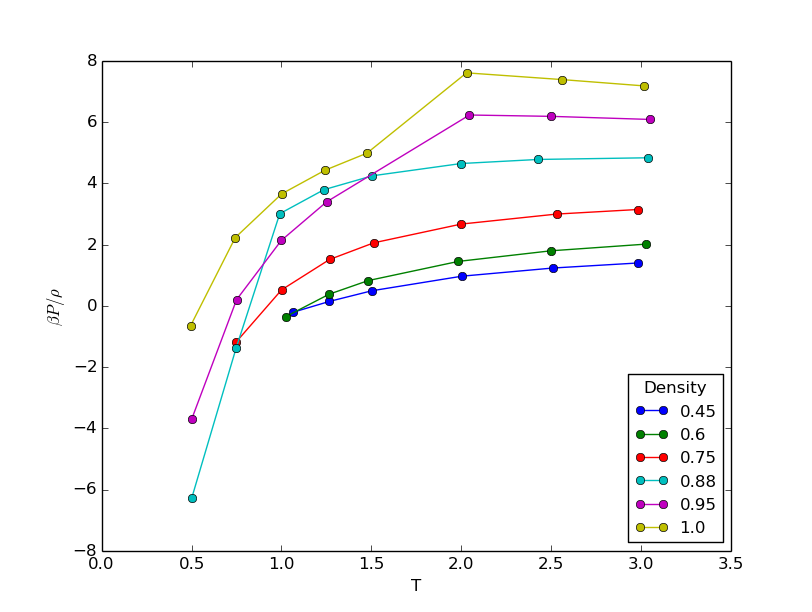
\includegraphics[scale=0.4]{pressure.png}
	\caption{Calculated pressure as a function of temperature for  several isochores\label{press_graph}}
\end{figure}

\subsection{Specific Heat}

\begin{figure}[ht]
	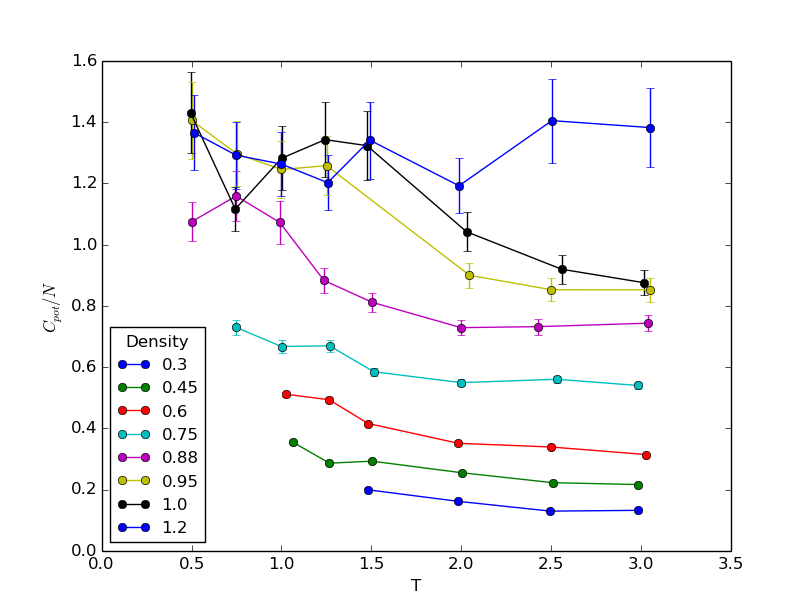
\includegraphics[scale=0.4]{heat_cap.png}
	\caption{Calculated potential specific heat per particle as a function of temperature for  several isochores (in units of $k_B$)\label{heat_cap_graph}}
\end{figure}

\section{Correlation function \label{correlation}}

\section{Decay of the velocity autocorrelation function \label{decay}}

\section{Conclusion \label{conclusion}}


% Create the reference section using BibTeX:
\bibliography{Sciences.bib}

\end{document}
